\documentclass[tikz,border=2pt]{standalone}
\usepackage{amsmath}
\usepackage{pgfplots}
\pgfplotsset{compat=1.18}
\usetikzlibrary{arrows.meta}
\begin{document}
% Epi(f) for f(x)=x^2 (shaded, unbounded above): the points (-1,1) and (2,4) lie in it, and their combination
% with weights 1/3 and 2/3 is (1,3), which lies in it because 1^2=1<=3.
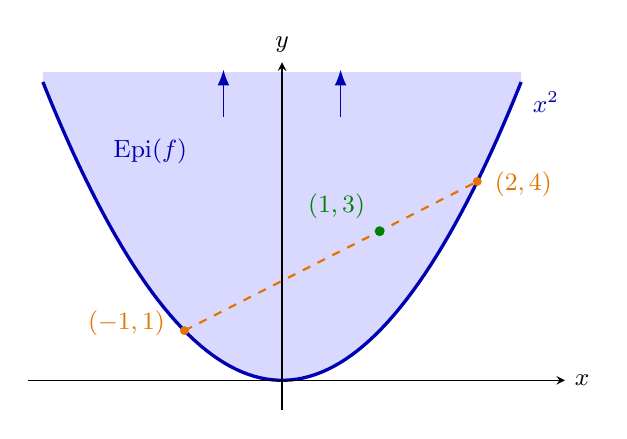
\begin{tikzpicture}[font=\small, >={Latex[length=2mm]}]
  \begin{axis}[
    axis lines=middle, xmin=-2.6, xmax=2.9, ymin=-0.6, ymax=6.4,
    xtick=\empty, ytick=\empty, axis on top,
    xlabel={$x$}, ylabel={$y$},
    xlabel style={anchor=west}, ylabel style={anchor=south},
    width=8.4cm, height=6cm, clip=false
    ]
    \addplot[draw=none, fill=blue!15, domain=-2.45:2.45, samples=80] {x^2} -- (axis cs:2.45,6.2) -- (axis cs:-2.45,6.2) -- cycle;
    \addplot[blue!70!black, very thick, domain=-2.45:2.45, samples=80] {x^2};
    \node[blue!70!black, anchor=west] at (axis cs:2.47,5.6) {$x^2$};
    \node[blue!70!black] at (axis cs:-1.35,4.6) {$\operatorname{Epi}(f)$};
    \draw[blue!70!black, ->] (axis cs:-0.6,5.3) -- (axis cs:-0.6,6.25);
    \draw[blue!70!black, ->] (axis cs:0.6,5.3) -- (axis cs:0.6,6.25);
    \draw[orange!90!black, thick, dashed] (axis cs:-1,1) -- (axis cs:2,4);
    \fill[orange!90!black] (axis cs:-1,1) circle (1.6pt);
    \fill[orange!90!black] (axis cs:2,4) circle (1.6pt);
    \node[orange!90!black, anchor=east] at (axis cs:-1.1,1.15) {$(-1,1)$};
    \node[orange!90!black, anchor=west] at (axis cs:2.08,3.95) {$(2,4)$};
    \fill[green!50!black] (axis cs:1,3) circle (1.8pt);
    \node[green!50!black, anchor=south east] at (axis cs:0.95,3.05) {$(1,3)$};
  \end{axis}
\end{tikzpicture}
\end{document}
